
%%% Local Variables:
%%% mode: latex
%%% TeX-master: t
%%% End:

\chapter{引言}
\label{cha:intro}

本章将介绍本文的相关背景,常用的凸包围体种类及应用,常见的碰撞检测算法及本文的结构安排。

\section{相关背景}

随着计算机软硬件的不断升级,人们的衣食住行越来越离不开计算机。
计算机图形学、计算机动画和虚拟现实等相关技术已经融入人类的日常生活当中,成为人们生活的重要组成部分,如虚拟手术、电影游戏等等。

凸包围体技术在计算机图形学的各种算法中发挥着重要作用,如优化渲染和建模,加速碰撞检测等。以求交算法为例,如果两个模型相交,则对应的凸包围体一定相交,若凸包围体不相交则原始模型一定不相交。凸包围体作为原始模型的近似,通常情况下,判断凸包围体是否相交比判断原始模型相交更简单,因此利用这个性质就可以加速模型之间的相交检测。
计算机图形学领域里常见的 AABB(Axis Aligned Bounding Box) 包围盒和计算几何领域里的凸包都是凸包围体。
凸包围体有多种应用,主要是利用其“凸”的性质及可用来近似被包含模型的特征,用于模型化简、碰撞检测等。在几何计算过程中,包围体也用于相交等操作中进行预判和剪枝以提升算法的运行效率。

碰撞检测问题是计算机图形学、虚拟现实等领域中的研究热点,是计算机模拟真实环境中不可或缺的技术,在物理仿真及游戏领域里应用广泛。例如在游戏中,碰撞检测保证了游戏的真实性,游戏角色不可穿墙、游戏中角色中弹而亡等等都离不开碰撞检测技术。

下面将分别介绍包围体相关技术和碰撞检测相关算法。

\section{凸包围体}
\label{sec:convexbv}

凸包围体之间的计算通常比包含的原始模型计算更简单,常用于在原始模型之间的相关计算(遮挡测试、相交测试等)进行预处理判断,当凸包围体之间没有相交或遮挡时,原始模型一定没有相交或遮挡。根据具体的应用场景的不同有不同形状的凸包围体,常见的如下。

\subsection{AABB 包围体}

AABB(Asix Aligned Bounding
Box)包围体是最常见最简单的包围体,俗称包围盒,其方向始终沿着坐标轴方向\cite{bergen1997efficient}。
在平面中就是包含二维模型的矩形,如图\ref{fig:aabb-bunny}所示,为平面图形~Bunny~的~AABB~包围体。对应到三维空间中就是沿坐标轴方向包含模型的最小的长方体。

\begin{figure}[H] % use float package if you want it here
  \centering
  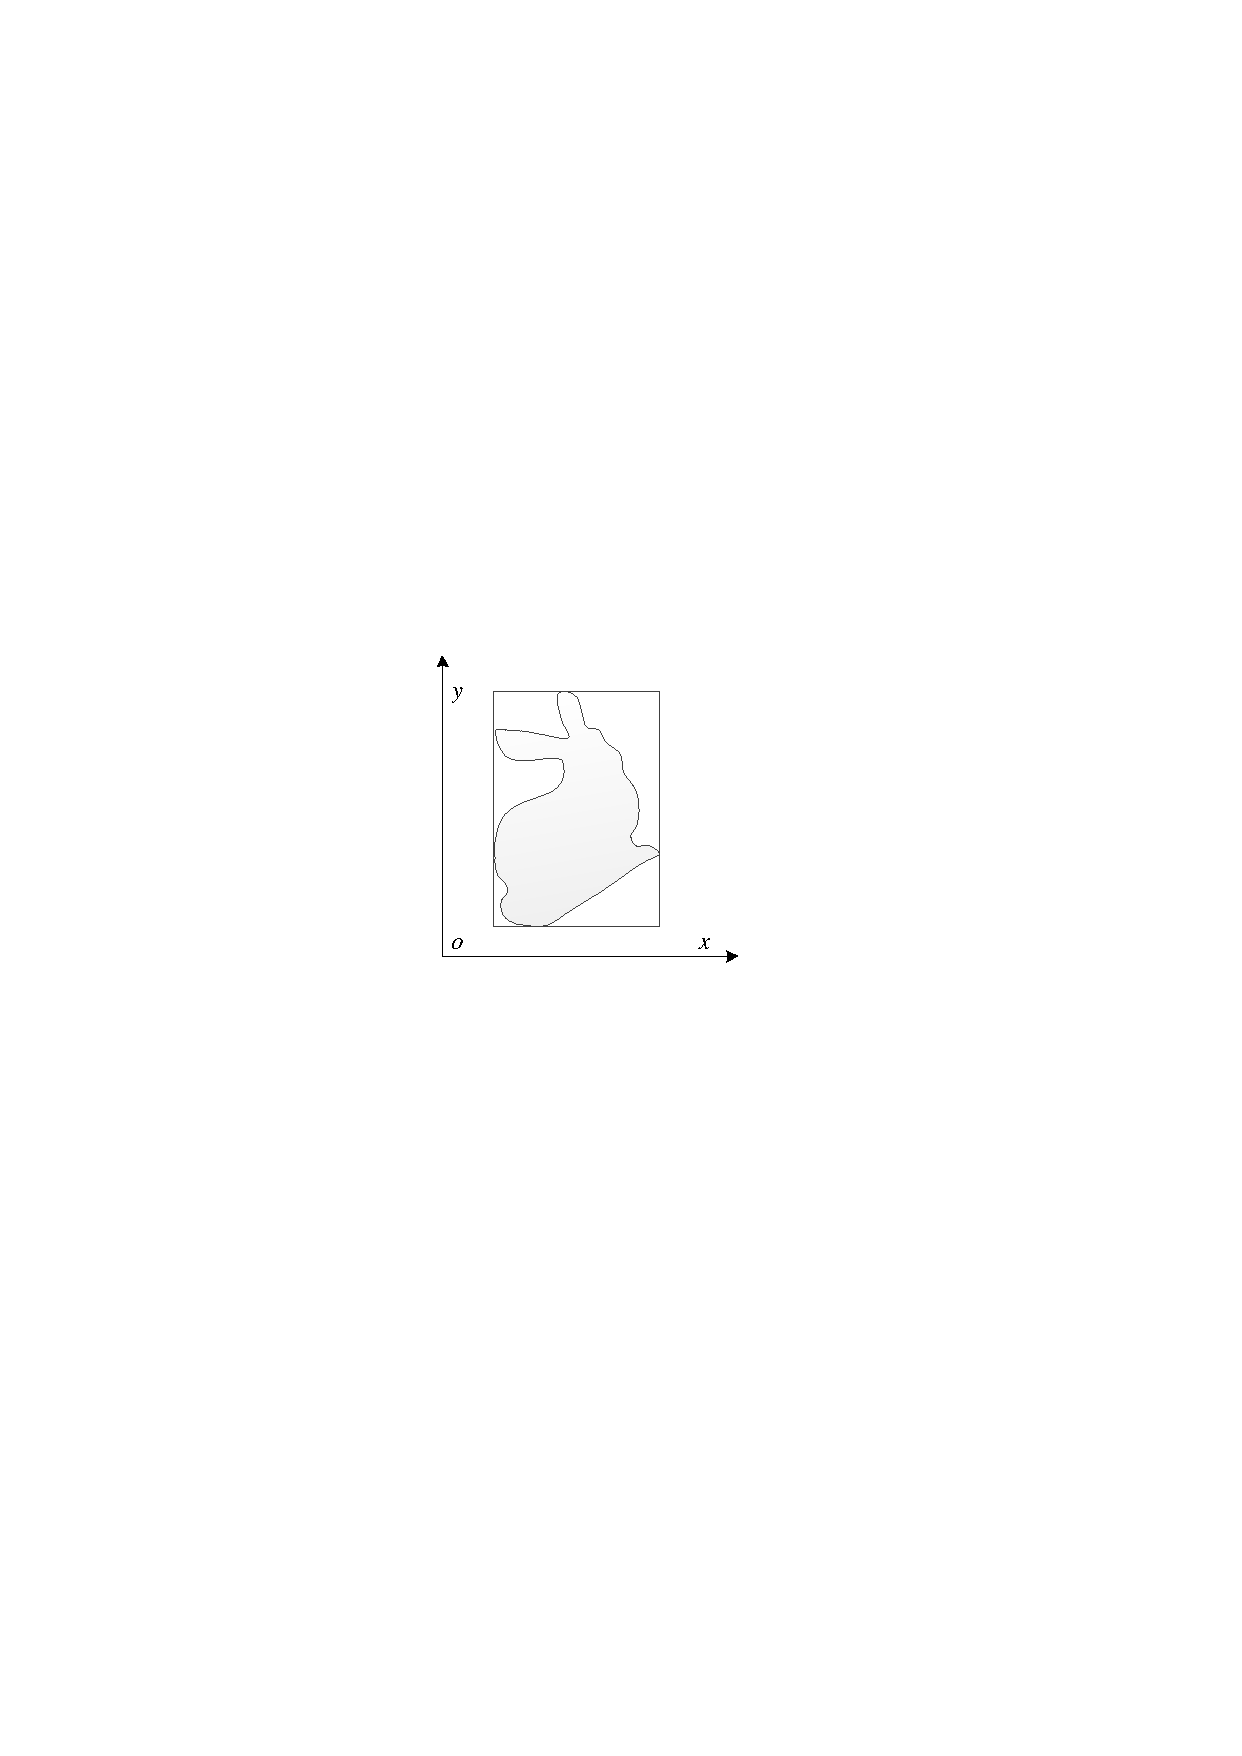
\includegraphics[width=1.5in]{bunny-2d-AABB.pdf}
  \caption{AABB 包围体}
  \label{fig:aabb-bunny}
\end{figure}

AABB~包围体的数据结构通常有3种方式:
\begin{inparaenum}[(1)]
\item 存储~AABB~包围体对角线上的两个极点,$Point_{min}$和$Point_{max}$,著名的计算几何库~CGAL\footnote{CGAL, Computational Geometry Algorithms Library, http://www.cgal.org}以此种方式存储;
\item 存储~AABB~包围体的中心点和各个方向的半径,$Point_{center}$和$Vector_{radius}$,如~SOLID\cite{bergen1997efficient};
\item 存储~AABB~包围体的极小点和各个方向的延伸长度\cite{ericson2005real},$Point_{min}$和$Vector_{extent}$。
\end{inparaenum} 

一方面~AABB~包围体之间的相交测试较简单,以数据结构为存储两个极点为例,只需要比较各个坐标值之间的大小即可。但另一方面,通常情况下与原始模型的近似性较差,因其包围体的边沿着坐标轴方向可能会留较多的空白空间。

\subsection{OBB 包围体}

~OBB(Oriented Bounding
Box)包围体是带方向的包围盒,可看作是~AABB~包围体沿任意方向转动一定角度后构成的包围体,因此通常情况下,~OBB~较~AABB~而言可以更紧致地贴近原始模型。
如图\ref{fig:obb-bunny}所示为平面图形~Bunny~的~OBB~包围体。

\begin{figure}[H] % use float package if you want it here
  \centering
  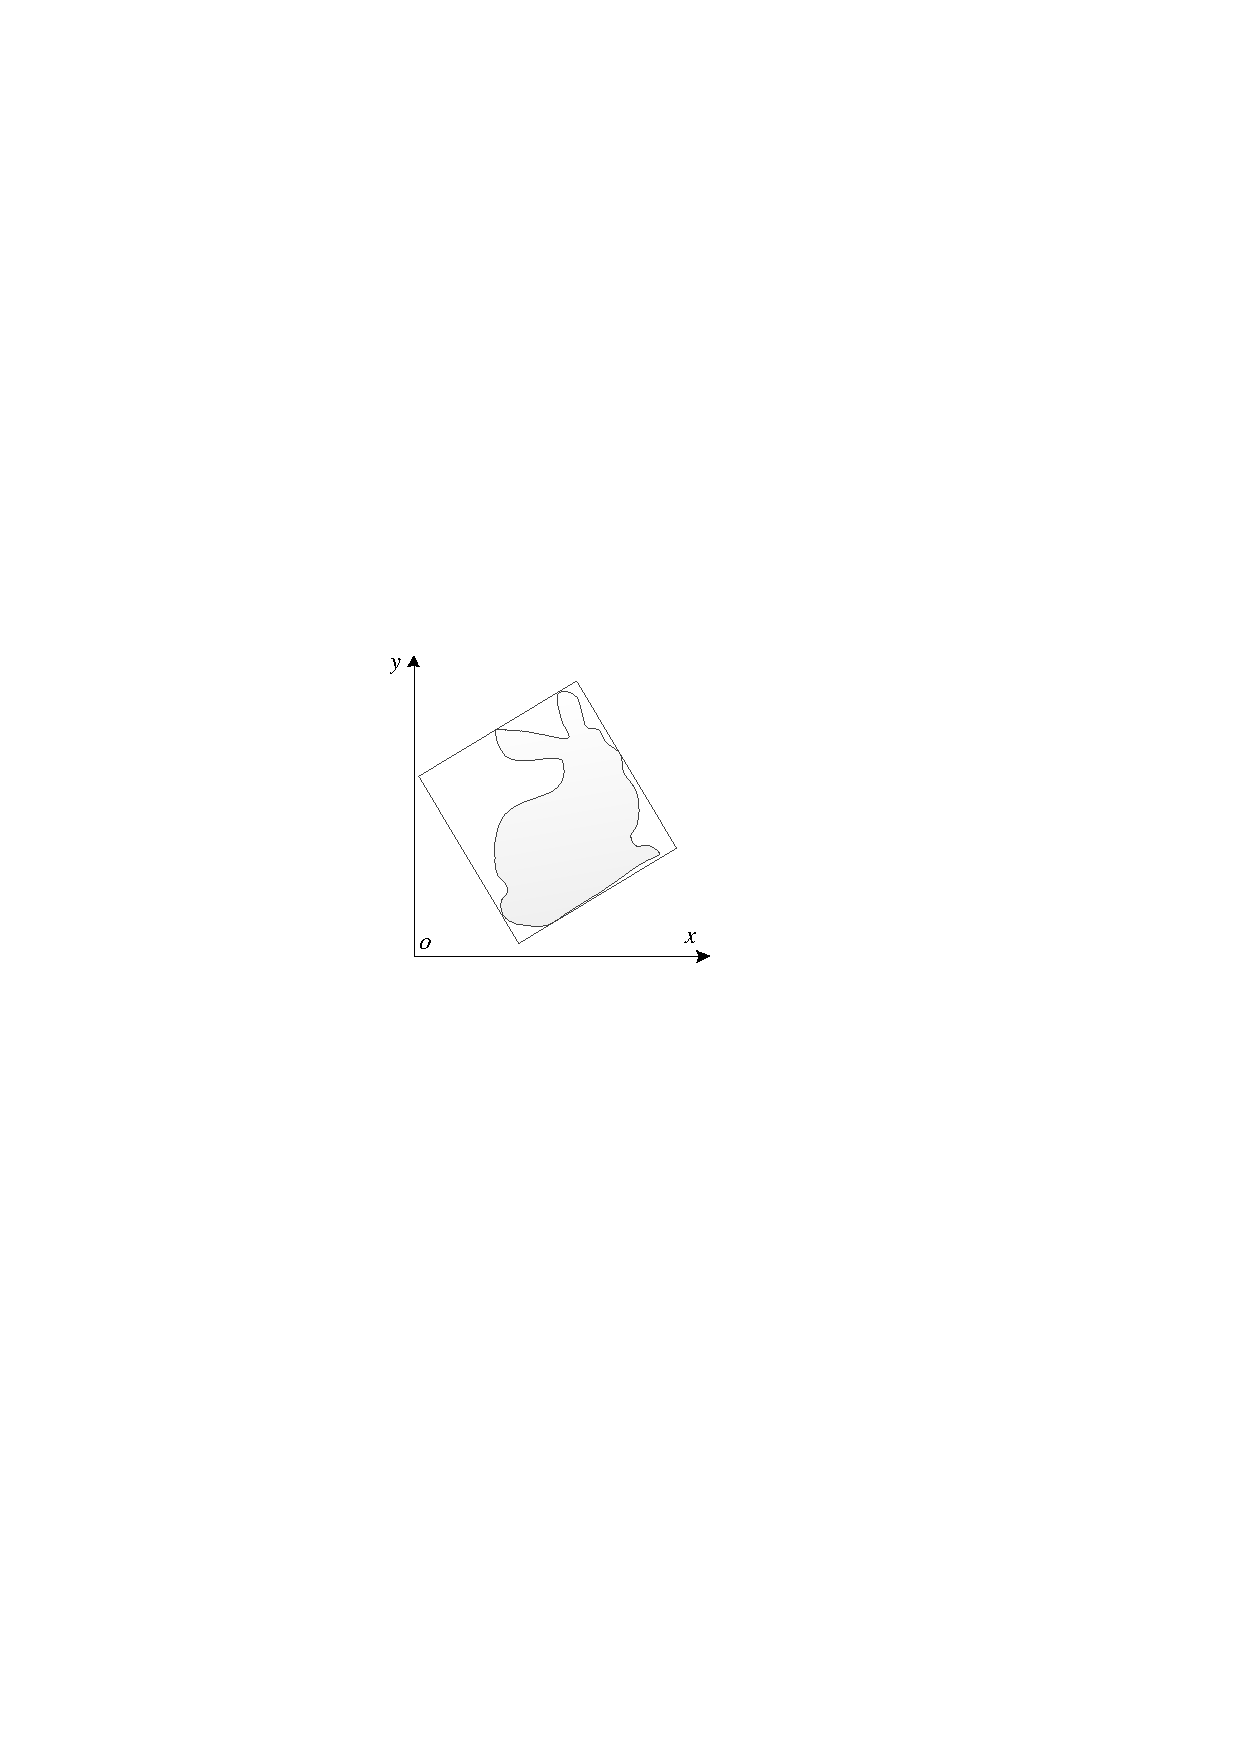
\includegraphics[width=1.5in]{bunny-2d-OBB.pdf}
  \caption{OBB 包围体}
  \label{fig:obb-bunny}
\end{figure}

与~AABB~类似,OBB~包围体的数据存储方式也可以有多种,最常用的是存储中心点,局部坐标架以及各个方向上的半径\cite{gottschalk1996obbtree}。因为~OBB~包围体的方向是任意的,有不少学者研究如何得到更加紧致的~OBB。
最早由~O'Rourke~\cite{o1985finding}提出了$O(n^3)$
算法,文献\onlinecite{barequet2001efficiently}中提出了一种方法理论上可以在$O(n
+ 1/ \epsilon ^{4.5} )$复杂度内计算出一个近似最小~OBB($\epsilon$
为近似误差,即得到的$V\leq(1+\epsilon)\times V_{min}$,
其中$V$表示~OBB~的体积),实际应用中通常实现的算法复杂度为$O(nlogn + n/
\epsilon ^{3} )$。~C.K.Chan~ \cite{chan2001determination}
提出了另外一种迭代的算法可以计算出误差范围内最小的~OBB~包围体,该算法适用于点数量较多(超过1万个点)的模型。

与~AABB~相比,~OBB~之间的相交测试稍复杂,需将二者转换到同一坐标系下进行计算,但其能更好的逼近原始模型。

\subsection{Sphere 包围体}

球形(Sphere)包围体,也称包围球(二维情况下即为包围圆,下同),即用一个半径尽量小的球包住给定所有点,该问题的求解是计算几何中的经典问题最小包围球的变种。
如图\ref{fig:sphere-bunny}所示为平面图形~Bunny~的包围圆。

\begin{figure}[H] % use float package if you want it here
  \centering
  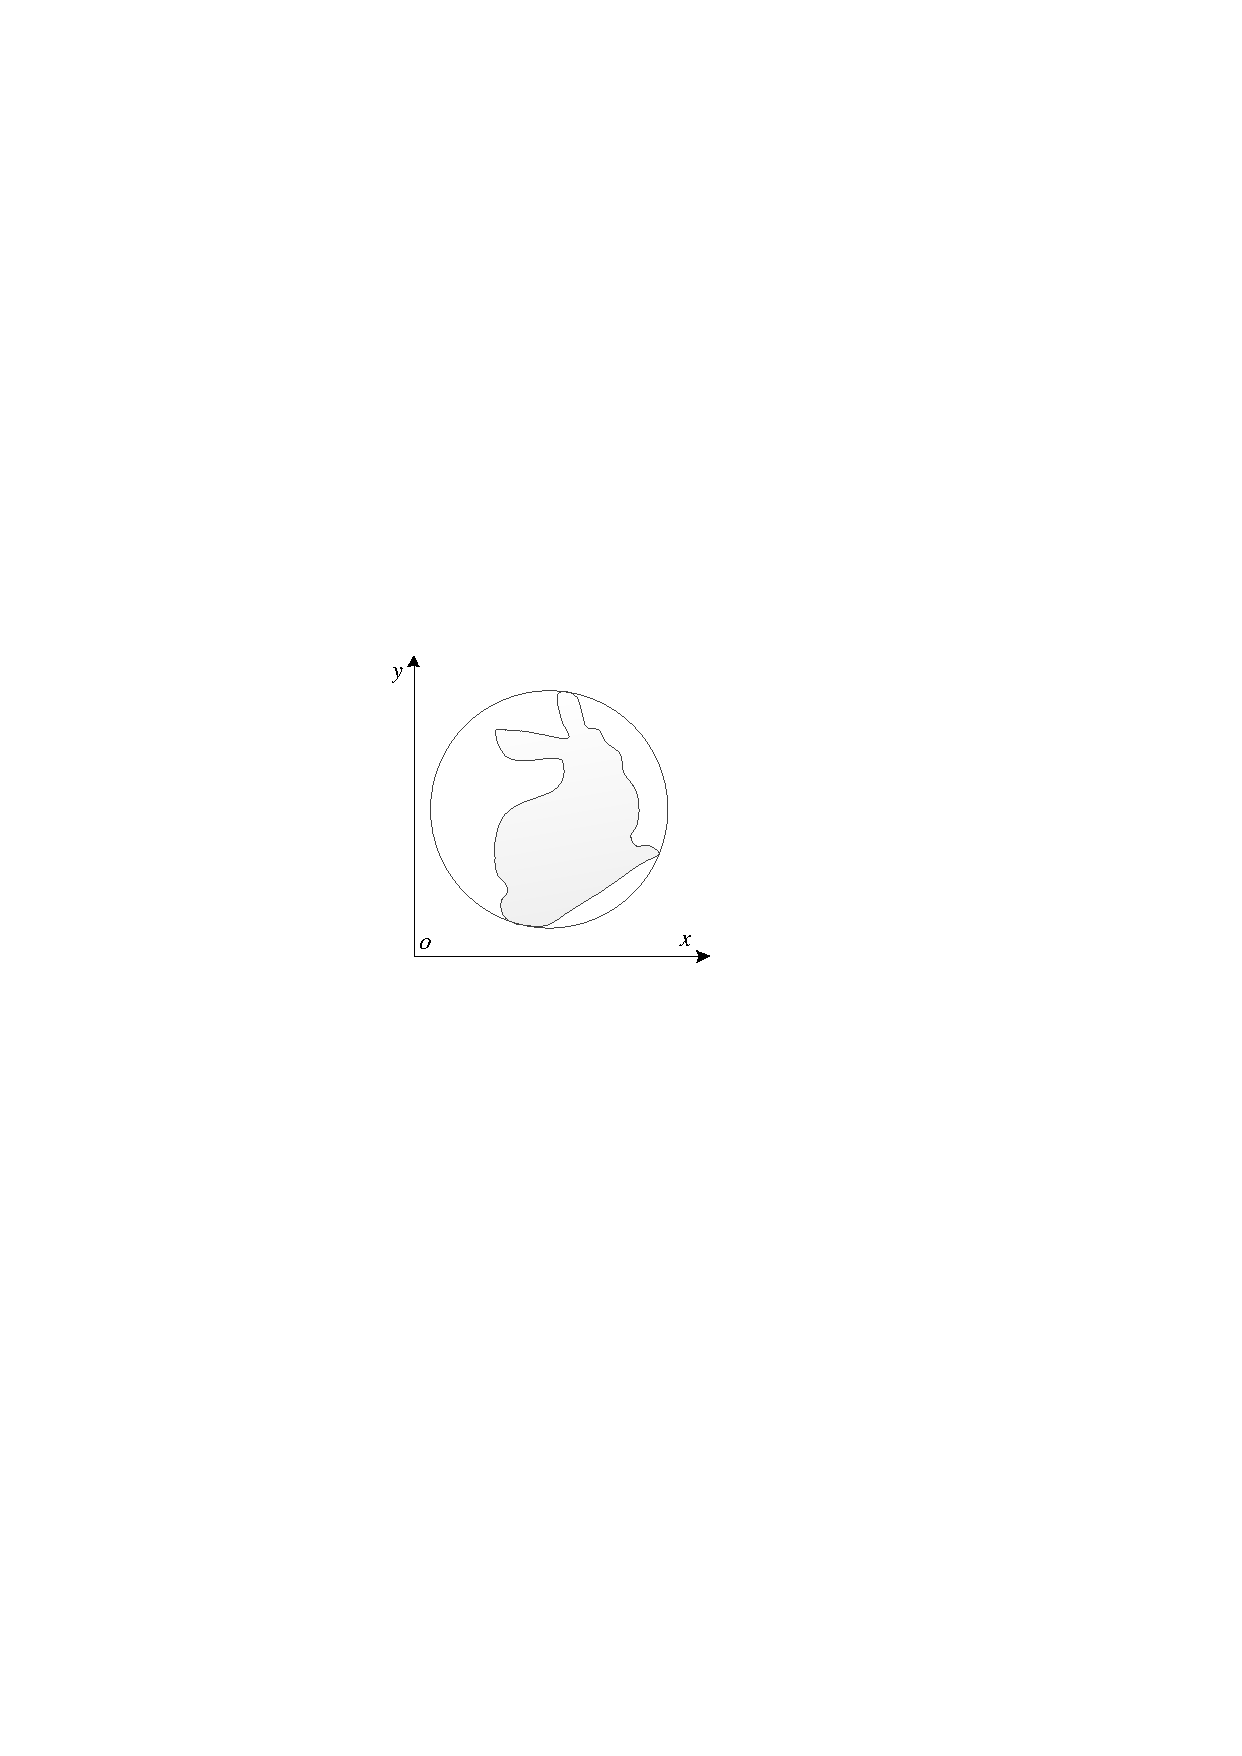
\includegraphics[width=1.5in]{bunny-2d-Sphere.pdf}
  \caption{Sphere 包围体}
  \label{fig:sphere-bunny}
\end{figure}

包围球的数据结构较简单,只需要球心和半径。一种最简单的计算一个包围求的方法是将相应~AABB~包围体的中心点作为球心,半径是为~AABB~各方向半径的最大值,这种方法虽然计算较快,但得到的包围体往往不够紧致。为了得到最小包围球,~E.Welzl~\cite{Welzl1991Smallest}
提出了一种线性的随机算法求出最小包围球。~T.Larsson~\cite{larsson2008fast}提出了一种快速简单的算法,该算法基于选择$k$个极点生成$k/2$个方向构造包围球,因而称为~EPOS~(Extremal Points Optimal Sphere~)算法,可以自定义$k$ 的值,能够给执行时间和包围盒紧致之间进行调整折衷,提高了灵活性。

测试两个包围球是否相交较简单,只需判断两个球心之间的距离是否大于两个球半径之和即可。

\subsection{$k$-DOP 包围体}

$k$-DOP(Discrete Orientation Polytope)包围体是一个由$k$个固定方向的半平面相交构成的凸多面体,其最早思想来源于~TL.Kay~\cite{Kay1986Ray}
等人提出的用于解决光线追踪的问题,~$k$-DOP~术语是由~J.Klosowski~等人\cite{klosowski1998efficient}
在1998 年用于解决碰撞检测问题时提出的,有学者也称~$k$-DOP~为$k$-FDH($k$-Fixed
Directions Hull)\cite{weiyingmei2001}。
在二维(三维)平面上,~k-DOP~就是一个由$k/2$对平行的固定方向的边(面)围成的凸多边形(多面体),其中$k\in\mathbb{N}$,$k\geq4$($k\geq6$)。如图\ref{fig:8dop-bunny}所示,为平面图形~Bunny~的$8$-DOP。

\begin{figure}[H] % use float package if you want it here
  \centering
  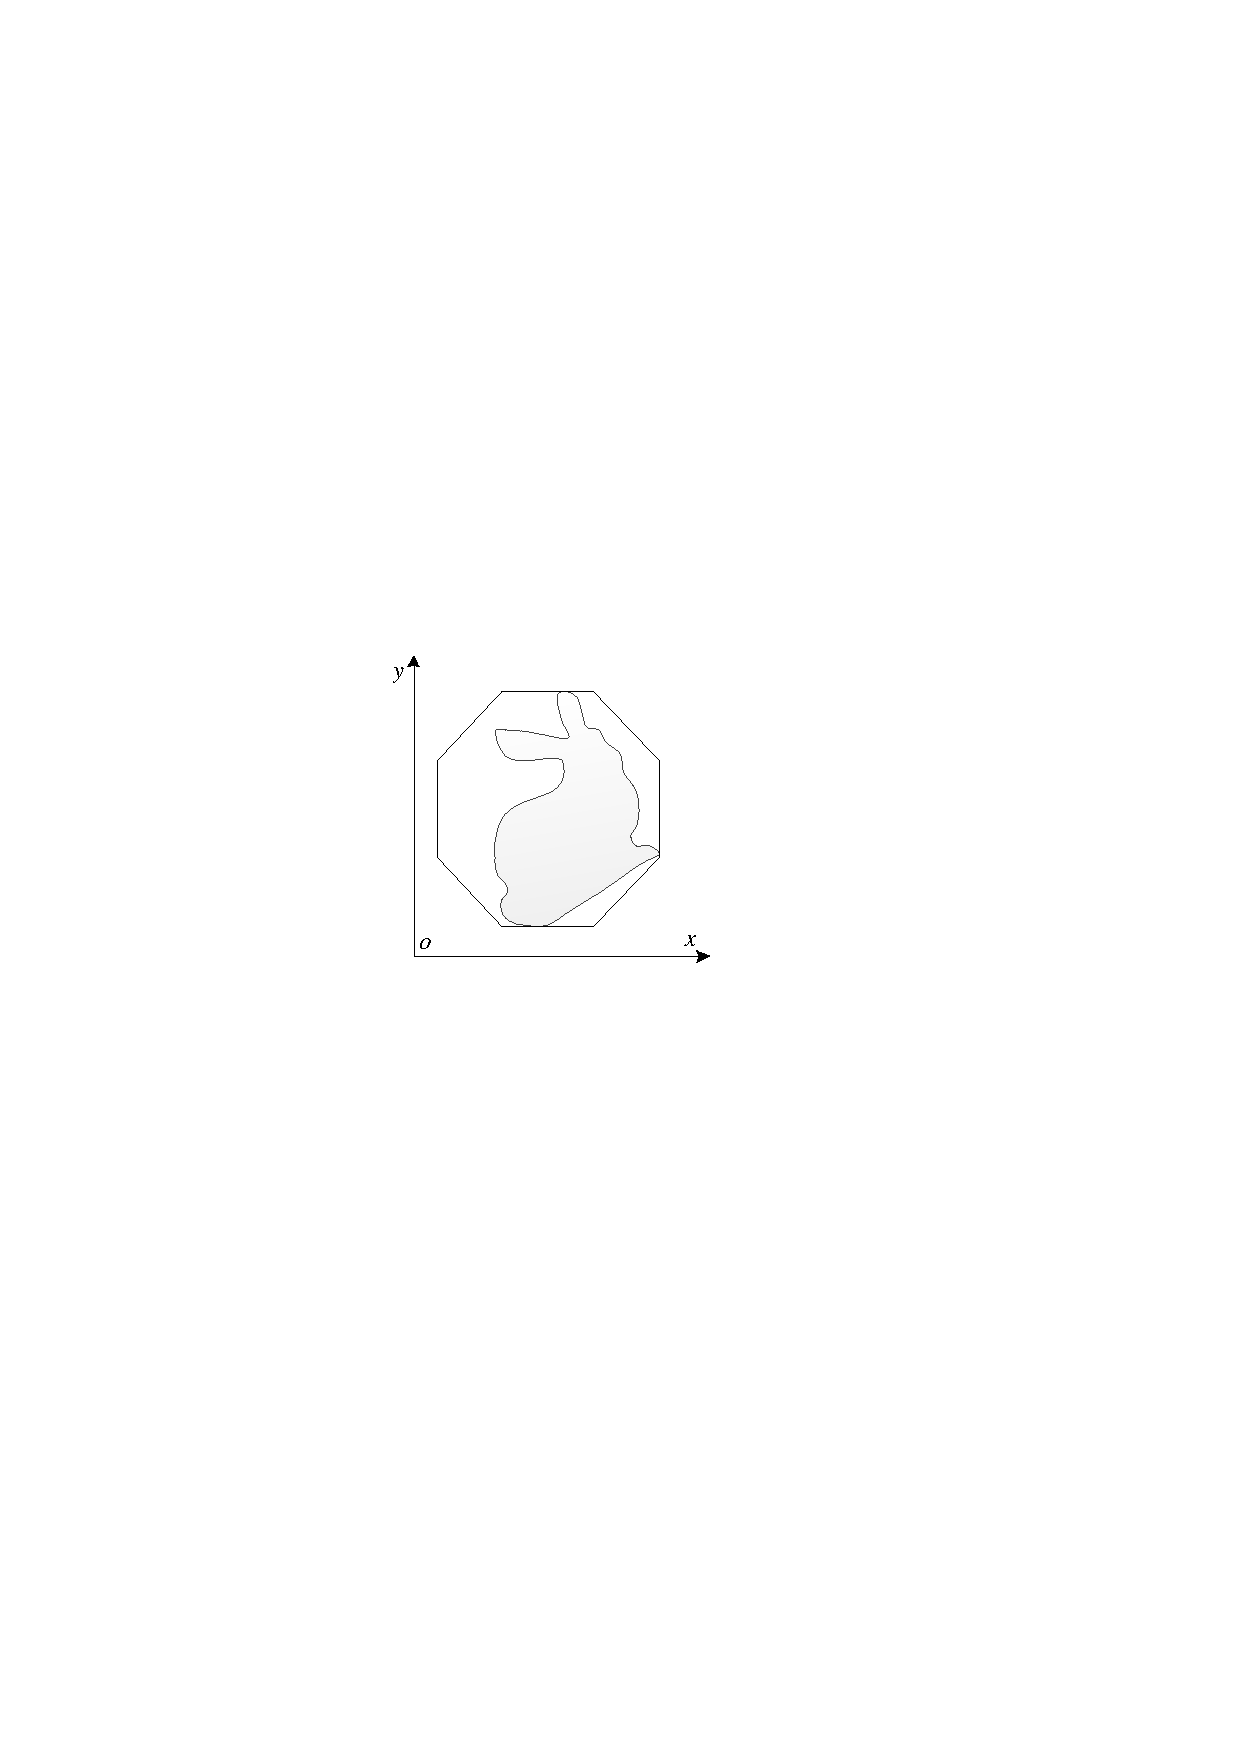
\includegraphics[width=1.5in]{bunny-2d-8DOP.pdf}
  \caption{$k$-DOP 包围体($k=8$)}
  \label{fig:8dop-bunny}
\end{figure}

对于$k$-DOP~中的每一个方向,可以由相应边(面)的法向决定,其数据结构一般用$k/2$个半平面的法向,再加上模型在各个方向上的投影的极值即可。因为$k$-DOP~的方向固定,$k$值确定后,相应的法向也随即确定,所以只需要存储各个方向的极值即可。当$k$-DOP~用于碰撞检测或可视化时,一般还需存储包围体的各个顶点。

与其他几种包围盒相比较而言,$k$-DOP~是取包围体存储计算和相交测试耗费时间的一个折衷,且可以通过修改$k$的值来提高包围体的灵活性。

\subsection{Convex hull 包围体}

凸包(Convex hull)是在计算几何中出现的概念,被定义为包含点集模型的最小凸集\cite{dengcg},
因此~Convex
hull~包围体是最紧致的凸包围体,能够更好地近似模型本身。
图\ref{fig:convexhull-bunny}为二维凸包的示例。

\begin{figure}[H] % use float package if you want it here
  \centering
  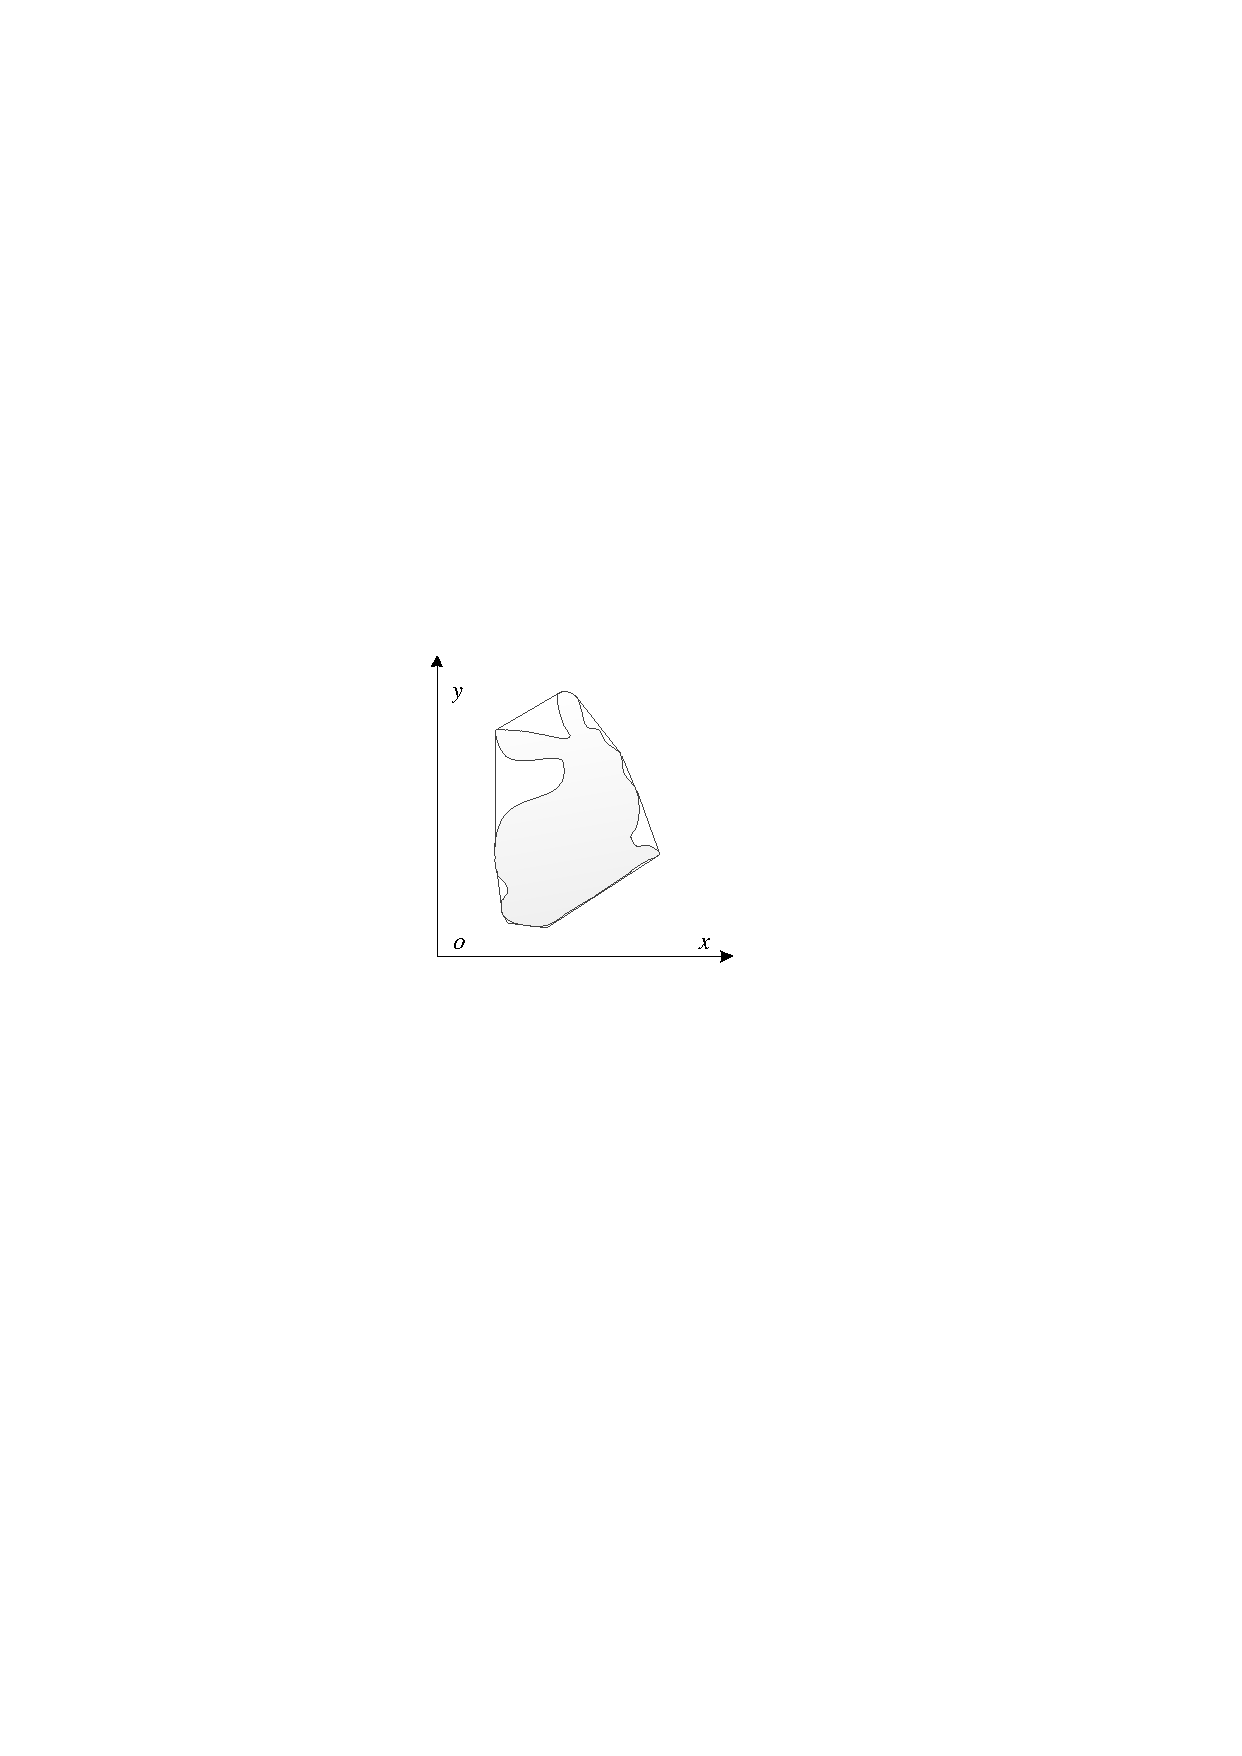
\includegraphics[width=1.5in]{bunny-2d-Convexhull.pdf}
  \caption{Convex hull 包围体}
  \label{fig:convexhull-bunny}
\end{figure}

常用的凸包构造算法有~Gift wrapping~\cite{Chand1970An},最坏情况下复杂度为$O(n^2)$,构造凸包的算法时间复杂度下限为$O(n\log n)$,如~Preparata~提出的分治算法\cite{Preparata1977}。
当模型点集较大时,包围体涉及到的面片数量太多,做相交测试等相关计算时耗费时间较久,同时也耗费较多存储空间。因此~Convex hull~包围体不太适用于大模型。
因此有学者在一些应用中用到近似凸包,
近似凸包可分为三类:近似外凸包、近似内凸包和近似凸包\cite{hossain2013constructing},
文献\onlinecite{bentley1982approximation,kavan2006fast}介绍了两种计算近似内凸包的算法,文
献\onlinecite{Zunie1992}介绍了一种计算二维近似外凸包算法。

\subsection{其他包围体}

除了以上几种常见的凸包围体外,不同学者在特定领域里也研究出以下另外几种包围体:\\
\begin{inparaenum}[(1)]
\indent
\item \textbf{Tribox} 可以看作是$k$-DOP~的一种特例,其中,二维中$k=8$ ,三维中$k=18$。 文献\onlinecite{crosnier1999tribox} 中提出的方法可以方便构造~Tribox~层次结构,并应用于模型分解中,当投影方向固定时,对于运动对象,更新其~Tribox~包围体也比较方便。 \\ 
\indent
\item \textbf{Swept-sphere}
是由~Eric.Larsen~等人\cite{Larsen1999Fast}提出的一种用于查询两个物体之间准确和近似相隔距离的解决方案,因而也用于碰撞检测的应用当中,该包围体有多种变种。原文中给出了球沿直线做拉伸构成的~Line-swept-sphere(如图\ref{fig:subfig-bv-swept-sphere}所示)
以及沿矩形拉伸构成的~Rectangle-swept-sphere~等阐述,并提出了构造层次结构包围体的算法,还对哪些包围体合适做碰撞检测,哪些包围体合适做最近距离计算做了分析和说明,更多内容可以参考文献\onlinecite{Larsen1999Fast}。\\
\indent
\item \textbf{Sphere-shell}
文献\onlinecite{krishnan1997spherical}给出了一种“球壳”(Sphere-shell)包围体,该包围体由两个同球心不同半径的球中间围成的壳与锥点为球心的锥面相交部分构成,如图\ref{fig:subfig-spherical-shell}所示。这种球壳包围体有利于非结构化的模型、多边形集合(Polygon
soups~)模型之间(如简单多边形,样条曲面构成的模型)的相隔距离计算或者进行碰撞检测。\\
\indent
\item \textbf{Zonotopes} 2003 年,~Leonidas
J.Guibas~\cite{Guibas2003Zonotopes}等人利用对偶的方法提出了一种用线段表示三维包围盒的隐式表达法,称其为~Zonotopes(二维称为~Zonogon),这种方法不用显示描述记录构成包围盒的多面体的每个面,节省存储,而同样能够在较快的时间内进行碰撞检测等。\\
\indent
\item \textbf{其他}
还有如图\ref{fig:subfig-bv-cylinder}所示的圆柱形\cite{Schomer2000Smallest}、图\ref{fig:subfig-bvcone}所示的圆锥形\cite{held1997erit}和如图\ref{fig:subfig-bv-ellipse}所示的椭球形\cite{Wang2004Efficient}等等包围体。
\end{inparaenum}

\begin{figure}[H]
  \centering%
  \subcaptionbox{圆柱形包围体\label{fig:subfig-bv-cylinder}}%[3cm] %标题的长度
    {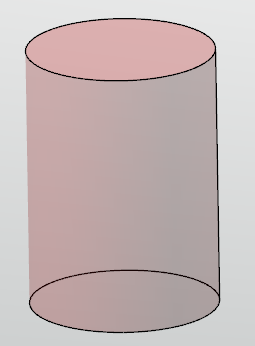
\includegraphics[height=4cm]{bv-cylinder.png}}
  \subcaptionbox{Sphere-shell~包围体\label{fig:subfig-spherical-shell}}
    {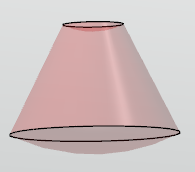
\includegraphics[height=4cm]{bv-spherical-shell.png}}
  \subcaptionbox{圆锥形包围体\label{fig:subfig-bvcone}}
    {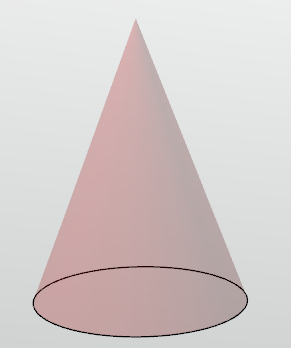
\includegraphics[height=4cm]{bv-cone.png}}
  \\
  \subcaptionbox{椭球形包围体\label{fig:subfig-bv-ellipse}}
    {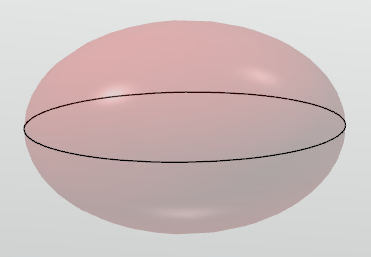
\includegraphics[height=4cm]{bv-ellipse.png}}
  \subcaptionbox{Swept-sphere~包围体\label{fig:subfig-bv-swept-sphere}}
    {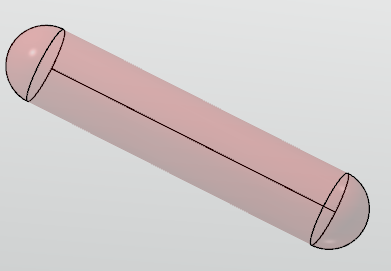
\includegraphics[height=4cm]{bv-swept-sphere.png}}
  \caption{其他包围体}
  \label{fig:bv-others}
\end{figure}

\subsection{包围体的应用}

包围体常见的应用领域有真实感渲染如可见面判别、视域剔除\cite{assarsson2000optimized},光线追踪\cite{wald2007ray}等。
在光线追踪算法中,包围体用于检测光线是否与物体相交,如果光线没有与包围体相交,则肯定不会与包围体内的物体模型相交,进而就不用渲染显示该物体。
另外更常见的应用就是碰撞检测\cite{wangzhiqiang1999},大多数碰撞检测算法都用到了各式各样的包围体以加速,如
\cite{larsson2006dynamic,madera2009hybrid,vogiannou2010enhancing,chang2010efficient,tang2010fast,zhigang2010efficient} 等。

有不少文献将包围体和模型简化技术结合起来,例如~Kai Huebner~等人\cite{huebner2008minimum}在利用文献
\onlinecite{barequet2001efficiently}中提出的构造最小~OBB~包围体算法的基础上将物体分解成多个~OBB~包围体,用这些~OBB~包围体近似原始模型用于机器人抓取中,如图\ref{lbl:Huebner2008-example}所示。类似的还有~Sphere~包围体的分解\cite{hubbard1996approximating}(如图\ref{lbl:hubbard1996approximating-example}),~Tribox~的分解\cite{crosnier1999tribox}等。

\begin{figure}[H]
  \centering
  \subcaptionbox{模型简化成~OBB~包围体\cite{huebner2008minimum}\label{lbl:Huebner2008-example}}%[3cm] %标题的长度
    {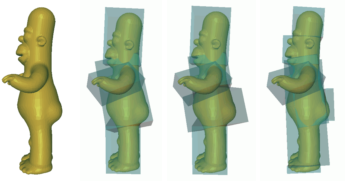
\includegraphics[height=4cm]{Huebner2008-example.png}}
  \subcaptionbox{模型简化成~Sphere~包围体\cite{hubbard1996approximating}\label{lbl:hubbard1996approximating-example}}
    {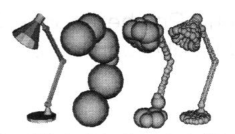
\includegraphics[height=4cm]{hubbard1996approximating-example.png}}
  \caption{包围体应用于模型简化}
  \label{lbl:bounding-voluems-used-in-shape-approximation}
\end{figure}

Jyh-Ming Lien~\cite{lien2006approximate2d}等人在06年提出一种方法可以将给定的多边形(包括含有孔洞的)分解成多个凸多边形,并提供不同种精度的分解,可以应用于~LoD~,并在07年将其扩展到三维\cite{lien2007approximate3d},即提出了一种方法将原始实体模型近似为层次结构的凸包围多面体,如图\ref{lbl:lien2007approximate-example} 所示,对图中的原始模型进行准确凸分解(~ECD,Exact Convex Decompositions~)将得到726240个组成部分,而近似凸分解(~ACD,Approximate Convex Decompositions~)仅得到98 个组成部分,同时保持了原始模型的大致形状,这大大加速了渲染过程。
\begin{figure}[H]
\centering
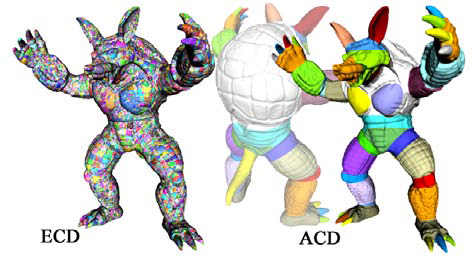
\includegraphics[width=3in]{lien2007approximate-example.png}
\caption{层次结构凸包围多面体的精确构造和近似构造\cite{lien2007approximate3d}}
\label{lbl:lien2007approximate-example}
\end{figure}
这种分解还可以应用于多种应用,例如运动规划(~Motion planning~),网格生成(~Mesh generation~),点定位(~Point location~)问题等等,更多内容可以参考\cite{lien2008approximate} 以及~Jyh-Ming Lien~ 的博士学位论文\cite{lien2006approximatephd}。

文献\cite{attene2008hierarchical}利用一种类似的方法将原始3D模型分解成一个具有层次结构的模型(图\ref{lbl:attene2008hierarchical-example:subfig1}所示),最顶层将是整个模型的凸包。将该算法应用到3D编辑环境中,能够更加方便地让用户选择模型的某个部分进行交互设计。效果如图\ref{lbl:attene2008hierarchical-example:subfig2} 所示,用户选择模型的头部,并进行拖拽能够较快速得到模型新的外观。\footnote{详情可参考视频:http://www.readcube.com/articles/10.1111/j.1467-8659.2008.01271.x }

\begin{figure}[H]
  \centering
  \subcaptionbox{层次结构的分解\label{lbl:attene2008hierarchical-example:subfig1}}
    {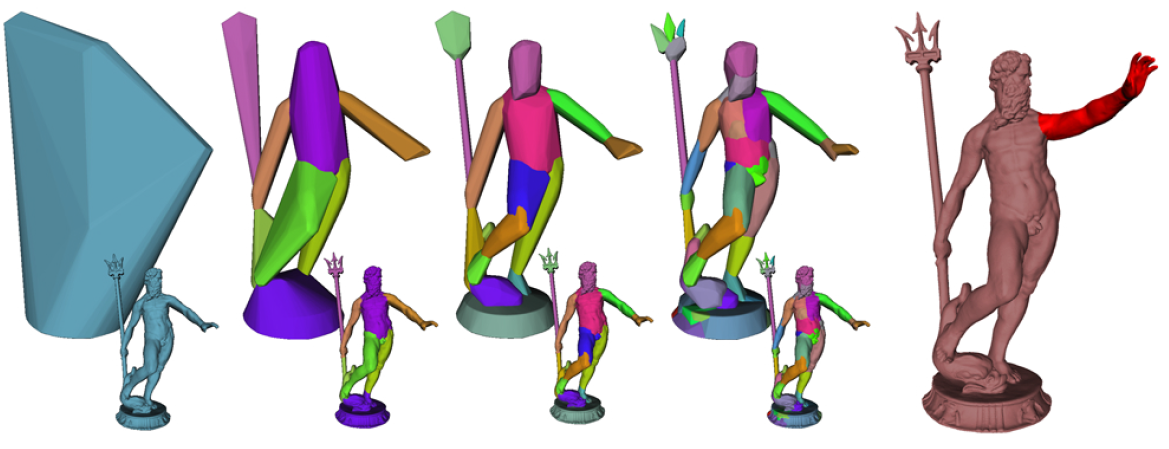
\includegraphics[height=2.8cm]{attene2008hierarchical-example-0.png}}
  \subcaptionbox{区域选择进行交互设计 \label{lbl:attene2008hierarchical-example:subfig2}}
    {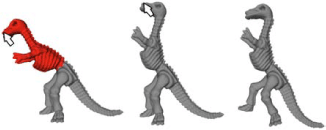
\includegraphics[height=2.8cm]{attene2008hierarchical-example.png}}
  \caption{层次结构的凸包围体及其应用于交互设计\cite{attene2008hierarchical}}
  \label{lbl:attene2008hierarchical-example}
\end{figure}

随着计算机软件技术和硬件的发展,有不少并行算法来计算包围体。
文献\cite{karlsson2010parallel}利用~Intel SIMD~(Single Instruction Multiple Data~,单指令多数据流)~SSE~指令集和~OpenMP~实现了对~AABB~,~OBB~和~$k$-DOP~的计算。
文献\cite{lauterbach2009fast}提出了在~CUDA~平台上基于~GPU~构造~AABB~包围体树的方法并应用于光线追踪。

\section{碰撞检测算法}
\label{sec:collisiondetection}

\subsection{碰撞检测算法的分类}
\label{sec:cd-category}


\subsection{基于包围体树的碰撞检测算法}
\label{sec:cd-bvh}

\section{本文主要内容}
\label{sec:structure}
论文组织结构

